\part{Solutions-to-Systems-of-DEs}
\lecture{Solutions to Systems of DEs}{Solutions-to-Systems-of-DEs}
\section{Solutions to Systems of DEs}


\title{Ordinary Differential Equations}
\subtitle{Math 232 - Solutions to Systems of Differential Equations}
\date{2 November 2012}

\begin{frame}
  \titlepage
\end{frame}

\begin{frame}
  \frametitle{Outline}
  \tableofcontents[pausesection,hideothersubsections]
\end{frame}


\subsection{Solutions to Systems of DEs}


\begin{frame}
  \frametitle{What is a solution to a System of DEs?}

  \begin{eqnarray*}
    \deriv{~}{t} \vec{x} & = & A \vec{x}.
  \end{eqnarray*}

  \uncover<2->
  {
    ``Looks'' like a first order, linear equation. The exponential has
    served us well in the past. Let's give it a try? Assume that 
    \begin{eqnarray*}
      \vec{x} & = & c e^{\lambda t} \vec{v}.
    \end{eqnarray*}
  }


\end{frame}


\begin{frame}
  \frametitle{Substitute it into the equation}

  The left hand Side:
  \begin{eqnarray*}
    \deriv{~}{t} \vec{x} & = & c \lambda e^{\lambda t} \vec{v} \\
  \end{eqnarray*}

  \uncover<2->
  {
    The right hand Side:
    \begin{eqnarray*}
      A \vec{x} & = & c e^{\lambda t} A \vec{v}.
    \end{eqnarray*}
  }

  \uncover<3->
  {
    Set them equal:
    \begin{eqnarray*}
      \Rightarrow c  e^{\lambda t} A \vec{v} & = & c \lambda e^{\lambda t} \vec{v}, \\
      A \vec{v} & = & \lambda \vec{v}.
    \end{eqnarray*}
  }

  \uncover<4->
  {
    This is an eigenvalue/eigenvector problem!
  }

\end{frame}


\begin{frame}
  \frametitle{Homogeneous Equations}

  Given
  \begin{eqnarray*}
    \deriv{~}{t} \vec{x} & = & A \vec{x},
  \end{eqnarray*}
  where $A$ is an $n\times n$ matrix, find the eigenvalues and
  eigenvectors. \textbf{If} there are \redText{$n$ linearly independent}
  eigenvectors then
  \begin{eqnarray*}
    \vec{x} & = & c_1 e^{\lambda_1 t} \vec{v}_1 + c_2 e^{\lambda_2 t} \vec{v}_2 +
    \cdot + c_n e^{\lambda_n t} \vec{v}_n.
  \end{eqnarray*}

\end{frame}

\subsection{Examples}

\iftoggle{clicker}{%
\begin{frame}
  \frametitle{Clicker Quiz}

   \ifnum\value{clickerQuiz}=1{%
\vfill


 }\fi

 \ifnum\value{clickerQuiz}=2{%
\vfill


 }\fi

 \ifnum\value{clickerQuiz}=3{%
  Given matrix 
  \begin{eqnarray*}
    A & = & \arrayTwo{5}{24}{-2}{-9}.
  \end{eqnarray*}
  Find the eigenvalues of $A$. 
  \begin{tabular}{ll}
          A: & $\lambda_1  = 5, \lambda_2 = -9$ \\
          B: & $\lambda_1  = -1, \lambda_2 = -3$ \\
          C: & $\lambda_1  = 2, \lambda_2 = -2$ \\
        \end{tabular}

  \vfill
 }\fi
\end{frame}
}


\begin{frame}
  \frametitle{Example}

  \begin{eqnarray*}
    \deriv{~}{t} \vec{x} & = & \arrayTwo{5}{24}{-2}{-9} \vec{x}.
  \end{eqnarray*}

  \uncover<2->
  {
    First find the eigenvalues,
    \begin{eqnarray*}
      0 & = & \det\lp\arrayTwo{5-\lambda}{24}{-2}{-9-\lambda}\rp, \\
      & = & (\lambda+1)(\lambda+3).
    \end{eqnarray*}
    The eigenvalues are \redText{$\lambda_1=-1$} and \blueText{$\lambda_2=-3$}.
  }

\end{frame}


\begin{frame}
  \frametitle{Find the eigenvectors}

  $\lambda_1 = -1$:
  \begin{eqnarray*}
    \arrayTwo{6}{24}{-2}{-8} \vecTwo{x}{y} & = & \vecTwo{0}{0}, \\
    6x + 24y & = & 0, \\
    -2x - 8y & = & 0, \\
    \uncover<2->
    {
      \Rightarrow \redText{\vec{v}_1} & \redText{=} & \redText{\vecTwo{-4}{1}}.
    }
  \end{eqnarray*}

  \uncover<3->
  {
    $\lambda_2 = -3$:
    \begin{eqnarray*}
      \arrayTwo{8}{24}{-2}{-6} \vecTwo{x}{y} & = & \vecTwo{0}{0}, \\
      8x + 24y & = & 0, \\
      -2x - 6y & = & 0, \\
      \uncover<4->
      {
        \Rightarrow \blueText{\vec{v}_2} & \blueText{=} & \blueText{\vecTwo{-3}{1}}.
      }
    \end{eqnarray*}
  }

\end{frame}


\begin{frame}
  \frametitle{Assemble the Solution}

  \begin{eqnarray*}
    \vec{x}(t) & = & \redText{c_1 e^{-t} \vecTwo{-4}{1}} + \blueText{c_2 e^{-3t} \vecTwo{-3}{1}}.
  \end{eqnarray*}

\end{frame}

\begin{frame}
  \frametitle{Example}

  \begin{eqnarray*}
    x'' + 5x' + 6x & = & 0, \\
    \Rightarrow x_h & = & C_1 e^{-3t} + C_2 e^{-2t}.
  \end{eqnarray*}

  \uncover<2->
  {
    Let $x'=y$,
    \begin{eqnarray*}
      x' & = & y, \\
      y' & = & -6x - 5y,
    \end{eqnarray*}
    which leads to the following system
    \begin{eqnarray*}
      \deriv{~}{t} \vec{x} & = & \arrayTwo{0}{1}{-6}{-5} \vec{x}.
    \end{eqnarray*}
  }

\end{frame}

\begin{frame}
    \frametitle{First find the eigenvalues}
    \begin{eqnarray*}
      0 & = & \det\lp\arrayTwo{-\lambda}{1}{-6}{-5-\lambda}\rp, \\
      & = & (\lambda+2)(\lambda+3).
    \end{eqnarray*}
    The eigenvalues are $\lambda_1=-2$ and $\lambda_2=-3$.

\end{frame}

\iftoggle{clicker}{%
\begin{frame}
  \frametitle{Clicker Quiz}

   \ifnum\value{clickerQuiz}=1{%
     \vfill
   }\fi

   \ifnum\value{clickerQuiz}=2{%
   \vfill
   }\fi

  \ifnum\value{clickerQuiz}=3{%
   For  $\lambda_1 = -2$, find the corresponding eigenvectors.
   \begin{tabular}{ll}
          A: & $\vec{v}_1  =  \vecTwo{1}{-2}.$ \\
          B: & $\vec{v}_1  =  \vecTwo{2}{1}.$ \\
          C: & $\vec{v}_1  =  \vecTwo{1}{2}.$ \\
        \end{tabular}

  \vfill
 }\fi
\end{frame}
}


\begin{frame}
  \frametitle{Find the eigenvectors}

  $\lambda_1 = -2$:
  \begin{eqnarray*}
    \arrayTwo{2}{1}{-6}{-3} \vecTwo{x}{y} & = & \vecTwo{0}{0}, \\
    2x + y & = & 0, \\
    -6x - 3y & = & 0, \\
    \uncover<2->
    {
      \Rightarrow \redText{\vec{v}_1} & \redText{=} & \redText{\vecTwo{1}{-2}}.
    }
  \end{eqnarray*}

  \uncover<3->
  {
    $\lambda_2 = -3$:
    \begin{eqnarray*}
      \arrayTwo{3}{1}{-6}{-2} \vecTwo{x}{y} & = & \vecTwo{0}{0}, \\
      3x + y & = & 0, \\
      -6x - 2y & = & 0, \\
      \uncover<4->
      {
        \Rightarrow \blueText{\vec{v}_2} & \blueText{=} & \blueText{\vecTwo{1}{-3}}.
      }
    \end{eqnarray*}
  }

\end{frame}


\begin{frame}
  \frametitle{Assemble the Solution}

  \begin{eqnarray*}
    \vec{x}(t) & = & \redText{c_1 e^{-2t} \vecTwo{1}{-2}} + \blueText{c_2 e^{-3t} \vecTwo{1}{-3}}.
  \end{eqnarray*}

  \uncover<2->
  {
    The Phase Plane:\\
    \centerline{\includegraphics[width=4cm]{img/phasePlaneExample}}

  }
  

\end{frame}


\begin{frame}
  \frametitle{Solution Behaviors and Nomenclature}

  \begin{columns}
    \column{.33\textwidth} \includegraphics[width=3cm]{img/phasePlaneSink}
    \column{.33\textwidth} \includegraphics[width=3cm]{img/phasePlaneSource}
    \column{.33\textwidth} \includegraphics[width=3cm]{img/phasePlaneSaddle}
  \end{columns}  

\end{frame}


\subsection{Repeated Eigenvalues}
\begin{frame}
  \frametitle{Example}
  \begin{eqnarray*}
    \deriv{~}{t} \vec{x} & = & \arrayTwo{2}{0}{0}{2} \vec{x}.
  \end{eqnarray*}
  \uncover<2->
  {
    Find the eigenvalues,
    \begin{eqnarray*}
      0 & = & \det\lp\arrayTwo{2-\lambda}{0}{0}{2-\lambda}\rp, \\
      & = & (2-\lambda)^2.
    \end{eqnarray*}
    The eigenvalue is $\lambda=2$.
  }
\end{frame}

\begin{frame}
  \frametitle{Find the Eigenvector}
  $\lambda_1=2$:
  \begin{eqnarray*}
    \arrayTwo{0}{0}{0}{0} \vecTwo{x}{y} & = & \vecTwo{0}{0}, \\
    \uncover<2->
    {
      \Rightarrow \vec{v} & = & \vecTwo{x}{y}, \\
      & = & x \vecTwo{1}{0} + y \vecTwo{0}{1}, \\
      \uncover<3->
      {
        \vec{v}_1 & = & \vecTwo{1}{0}, \\
        \vec{v}_2 & = & \vecTwo{0}{1}.
      }
    }
  \end{eqnarray*}
\end{frame}

\begin{frame}
  \frametitle{Form the Solution}
  The solution is
  \begin{eqnarray*}
    \vec{x} & = & c_1 e^{2t} \vecTwo{1}{0} + c_2 e^{2t} \vecTwo{0}{1}.
  \end{eqnarray*}
\end{frame}


\begin{frame}
  \frametitle{Example}

  \begin{eqnarray*}
    \deriv{~}{t} \vec{x} & = & \arrayTwo{0}{-1}{4}{-4} \vec{x}.
  \end{eqnarray*}

  \uncover<2->
  {
    Find the eigenvalues:
    \begin{eqnarray*}
      0 & = & \det\lp\arrayTwo{-\lambda}{-1}{4}{-4-\lambda}\rp, \\
      & = & \lp \lambda + 2 \rp^2,
    \end{eqnarray*}
    The value of $\lambda$ is -2.
  }

\end{frame}


\begin{frame}
  \frametitle{Find the eigenvectors}

  \begin{eqnarray*}
    \arrayTwo{2}{-1}{4}{-2} \vec{x}{y} & = & \vecTwo{0}{0}, \\
    2x - y & = & 0, \\
    4x - 2y & = & 0.
  \end{eqnarray*}

  There is only one eigenvector,
  \begin{eqnarray*}
    \vec{v}_1 & = & \vecTwo{1}{2}.
  \end{eqnarray*}
  One homogeneous solution is 
  \begin{eqnarray*}
   \vec{x}_1 & = & e^{-2t}\vecTwo{1}{2}.
  \end{eqnarray*}

\end{frame}

\begin{frame}
  \frametitle{What to do?}

  Last time this happened we tried to multiply by $t$, and it
  worked. We will try that again...
  Assume that
  \begin{eqnarray*}
    \vec{x} & = & t e^{\lambda t} \vec{v} + e^{\lambda t} \vec{u}.
  \end{eqnarray*}

  \uncover<2->
  {
    Substitute back into the equation:
    \begin{eqnarray*}
      \deriv{~}{t} \vec{x} & = & \lambda t e^{\lambda t} \vec{v} + e^{\lambda t} \vec{v} 
         + \lambda e^{\lambda t} \vec{u}, \\
      A\vec{x} & = & t e^{\lambda t} A \vec{v} + e^{\lambda t} A \vec{u}.
    \end{eqnarray*}
  }
  
\end{frame}


\begin{frame}
  \frametitle{Set The Two Expressions Equal}

  \only<1>
  {
    \begin{eqnarray*}
      \lambda t e^{\lambda t} \vec{v} + e^{\lambda t} \vec{v} + \lambda e^{\lambda t} \vec{u}
      & = & 
      t e^{\lambda t} A \vec{v} + e^{\lambda t} A \vec{u}.
    \end{eqnarray*}
  }

  \only<2->
  {
    \begin{eqnarray*}
      \redText{\underbrace{\lambda t e^{\lambda t} \vec{v}}_ {te^{\lambda t}}} +  
      \blueText{\underbrace{e^{\lambda t} \vec{v} + \lambda e^{\lambda t} \vec{u}}_{e^{\lambda t}}}
      & = & 
      \redText{\underbrace{t e^{\lambda t} A \vec{v}}_{t e^{\lambda t}}} + 
      \blueText{\underbrace{e^{\lambda t} A \vec{u}}_{e^{\lambda t}}}.
    \end{eqnarray*}

    Match the like terms.

  }
  

\end{frame}

\begin{frame}
  \frametitle{Set The Two Expressions Equal}

    \begin{eqnarray*}
      \redText{\lambda t e^{\lambda t} \vec{v}} + \blueText{e^{\lambda t} \vec{v} + \lambda e^{\lambda t} \vec{u}}
      & = & 
      \redText{t e^{\lambda t} A \vec{v}} + \blueText{e^{\lambda t} A \vec{u}}.
    \end{eqnarray*}
  
    This has to be true for all $t$ so we have the following equations:
    \begin{eqnarray*}
      \redText{\lambda t e^{\lambda t} \vec{v}} & \redText{=} & \redText{t e^{\lambda t} A \vec{v}}, \\
      \lambda \vec{v} & = & A \vec{v}.
    \end{eqnarray*}
    (This is the eigenvalue and eigenvector!)

    We also have 
    \begin{eqnarray*}
      \blueText{e^{\lambda t} \vec{v} + \lambda e^{\lambda t} \vec{u}} & \blueText{=} & \blueText{e^{\lambda t} A \vec{u}} , \\
      \vec{v} + \lambda \vec{u} & = &  A \vec{u}, \\
      \Rightarrow \lp A - \lambda I \rp \vec{u} & = & \vec{v}.
    \end{eqnarray*}

\end{frame}


\begin{frame}
  \frametitle{Back to the Example}

  \begin{eqnarray*}
    \deriv{~}{t} \vec{x} & = & \arrayTwo{0}{-1}{4}{-4} \vec{x}.
  \end{eqnarray*}


  There is only one eigenvalue, $\lambda=-2$ with one eigenvector,
  \begin{eqnarray*}
    \vec{v}_1 & = & \vecTwo{1}{2}.
  \end{eqnarray*}
  One homogeneous solution is 
  \begin{eqnarray*}
   \vec{x}_1 & = & e^{-2t}\vecTwo{1}{2}.
  \end{eqnarray*}


\end{frame}


\begin{frame}
  \frametitle{Finding the other solution}

  Assume a solution in the form
  \begin{eqnarray*}
    \vec{x} & = & t e^{-2 t} \vecTwo{1}{2} + e^{-2 t} \vec{u}, \\
    \arrayTwo{2}{-1}{4}{-2} \vecTwo{x}{y} & = & \vecTwo{1}{2}, \\
    2x-y & = & 1 \\
    4x-2y & = & 2.
  \end{eqnarray*}

  The vector, $\vec{u}$, is the following:
  \begin{eqnarray*}
    \vec{u} & = & \vecTwo{0}{-1}+\vecTwo{1}{2}x. 
  ~~~~\text{Let }  \vec{u}  =  \vecTwo{0}{-1}.
  \end{eqnarray*}
  One homogeneous solution is:
  \begin{eqnarray*}
    \vec{x}_2 & = & te^{-2t}\vecTwo{1}{2}+e^{-2t}\vecTwo{0}{-1} 
     =  e^{-2t}\vecTwo{t}{2t-1}.
  \end{eqnarray*}

\end{frame}

\begin{frame}
  \frametitle{Form the Solution}
  
  The solution to the differential equation is
  \begin{eqnarray*}
    \vec{x}(t) & = &  C_1 e^{-2t} \vecTwo{1}{2} + C_2 e^{-2t}\vecTwo{t}{2t-1}.
  \end{eqnarray*}
\end{frame}


\subsection{Coupled Tank Problems}


\begin{frame}
  \frametitle{Coupled Tank}

  \only<1>{\centerline{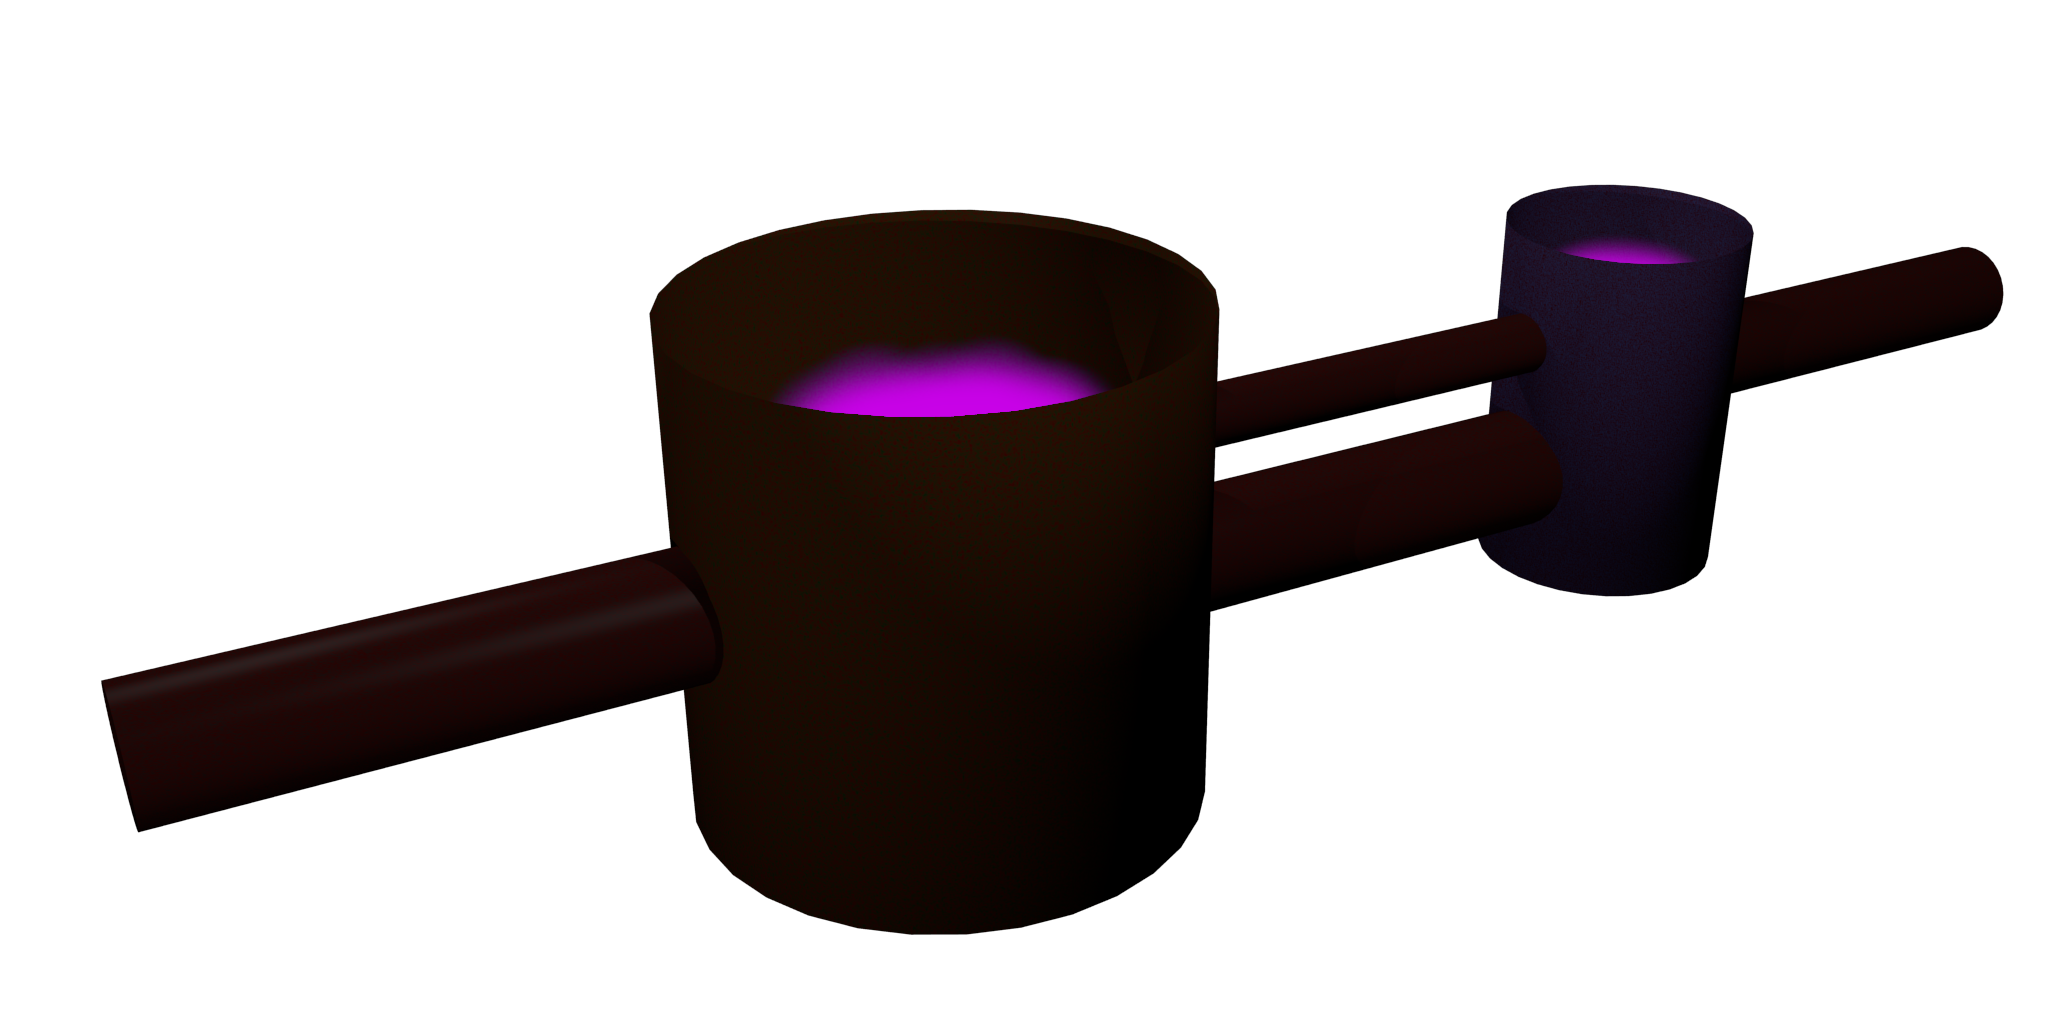
\includegraphics[width=9cm]{img/doubleTank}}}
  \only<2>{\centerline{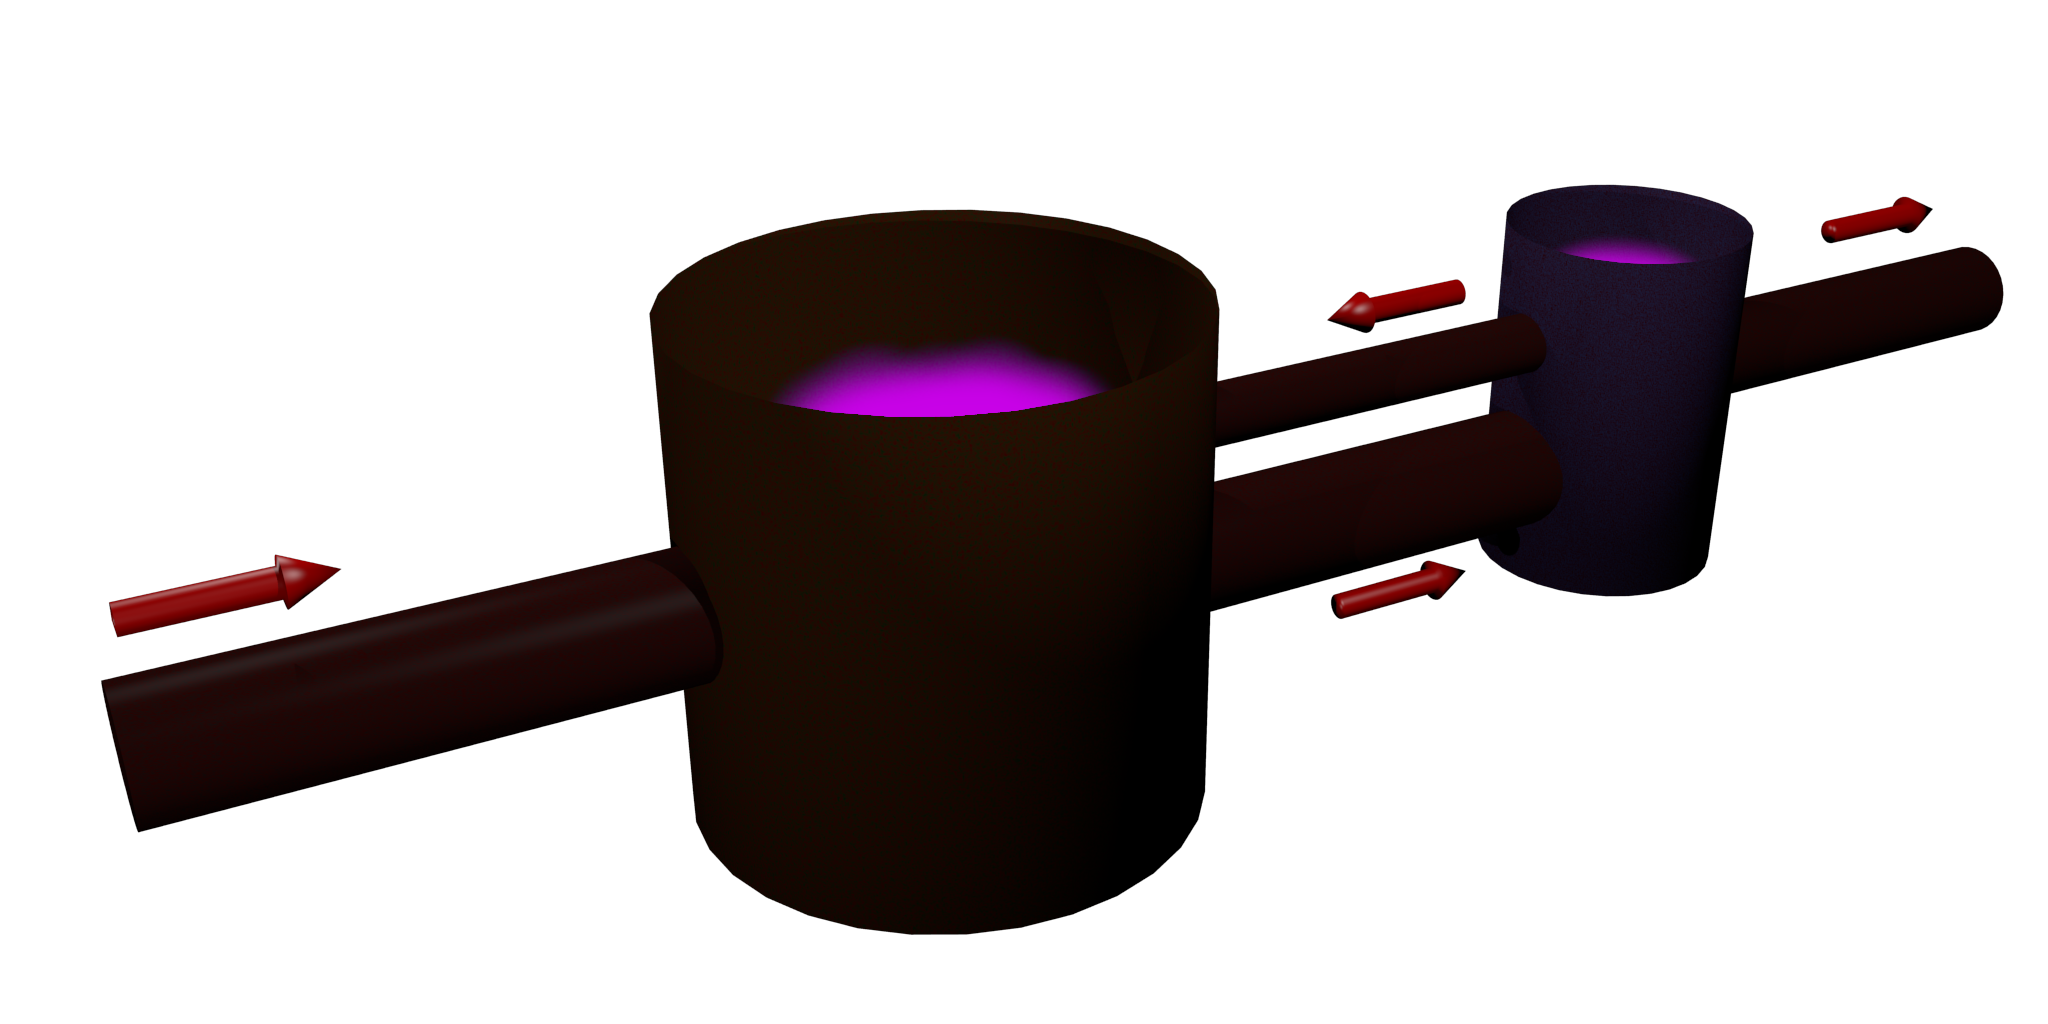
\includegraphics[width=9cm]{img/doubleTankArrows}}}
  \only<3>{\centerline{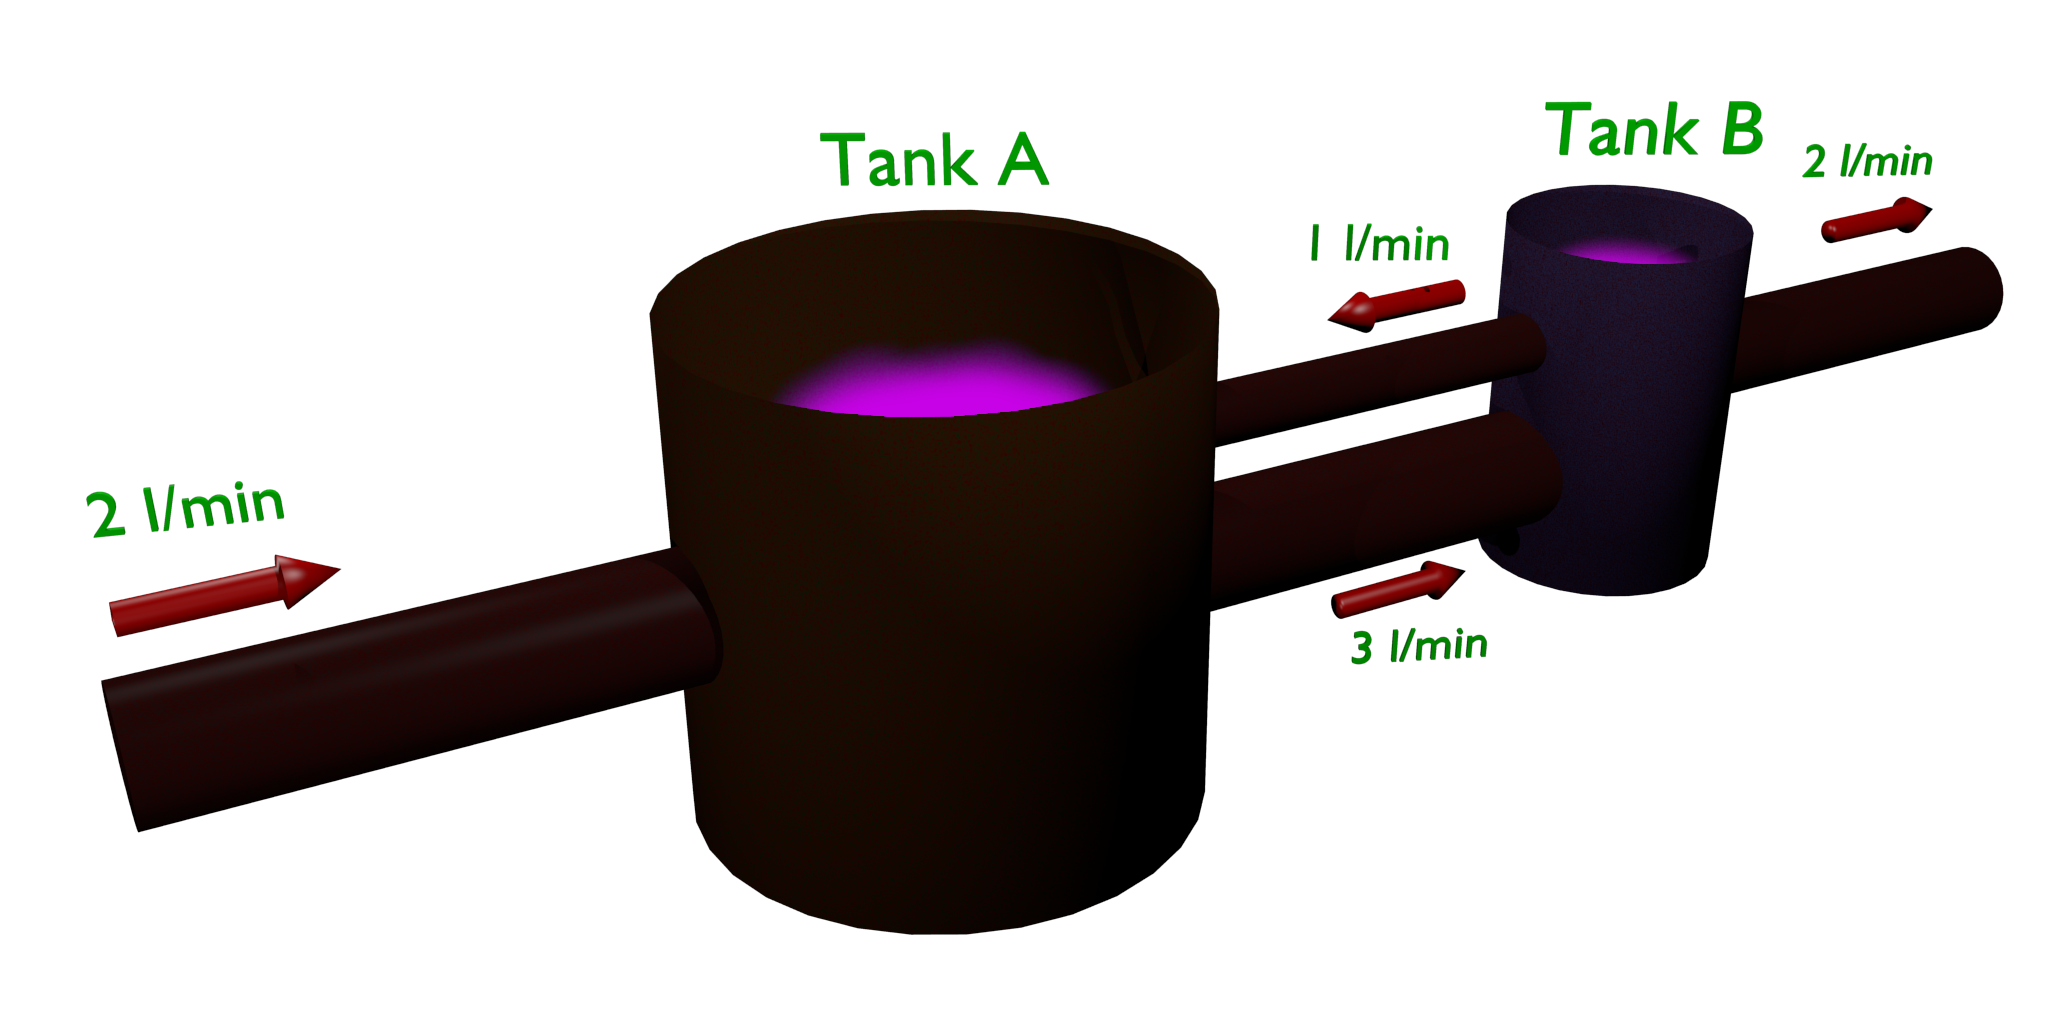
\includegraphics[width=9cm]{img/doubleTankAnnotated}}}

  Two tanks are arranged as shown. Initially tank A has 100 liters of
  water and tank B has 50 liters of water. Initially each tank has 2
  kg of salt dissolved in the solution. Pure water is pumped into to
  the first tank at a rate of 2 liters per minute. The solution in the
  second tank is pumped out a rate of 2 liters per minute. Determine
  the amount of salt in each tank at any time.
  
\end{frame}


\begin{frame}
  \frametitle{System of Equations}

  $x(t)$ is the amount of salt in tank A at time $t$.

  $y(t)$ is the amount of salt in tank B at time $t$.

  \begin{eqnarray*}
    \deriv{x}{t} & = & 0\times 2 - 
    \frac{x}{100}\times 3 + \frac{y}{50}\times 2 \\
    \deriv{y}{t} & = & \frac{x}{100} \times 3 -
    \frac{y}{50} \times 1 - \frac{y}{50}\times 2.
  \end{eqnarray*}

  Written as a system we get
  \begin{eqnarray*}
    \deriv{~}{t} \vecTwo{x}{y} & = & 
    \arrayTwo{-3/100}{2/50}{3/100}{-3/50} \vecTwo{x}{y}.
  \end{eqnarray*}
  
\end{frame}


% LocalWords:  Clarkson pausesection hideothersubsections eigenvector
% LocalWords:  eigenvectors
